% ASGARD/Loki draft (verified numbers, humanized)
\section{Automated Manuscript Assembly and QA Record}
\label{app:assembly}

This manuscript was assembled and quality-checked with the ASGARD Research Hub, a dual-persona agent system (Thor: literature positioning and adversarial review; Loki: drafting, humanisation and integrity control). The assembly pipeline is shown in Fig.~\ref{fig:assembly}. Every quantitative statement was locked to the repository's verified tables before drafting; the humanisation pass then verified that all key numbers, intervals and citations survived rewriting unchanged. The Thor council reviewed the abstract and contribution claims in two rounds with independent scoring; verdicts are summarised in the run report shipped alongside this paper. The integrity suite measured self-overlap across sections, citation coverage, notation consistency and coherence; the claim--evidence map (Appendix~\ref{app:claims}) traces every quantitative claim to its source file. The system's role is editorial and evidentiary: it does not generate results, and no number in this paper originates from the assembly layer.

\begin{figure}[htbp]
\centering
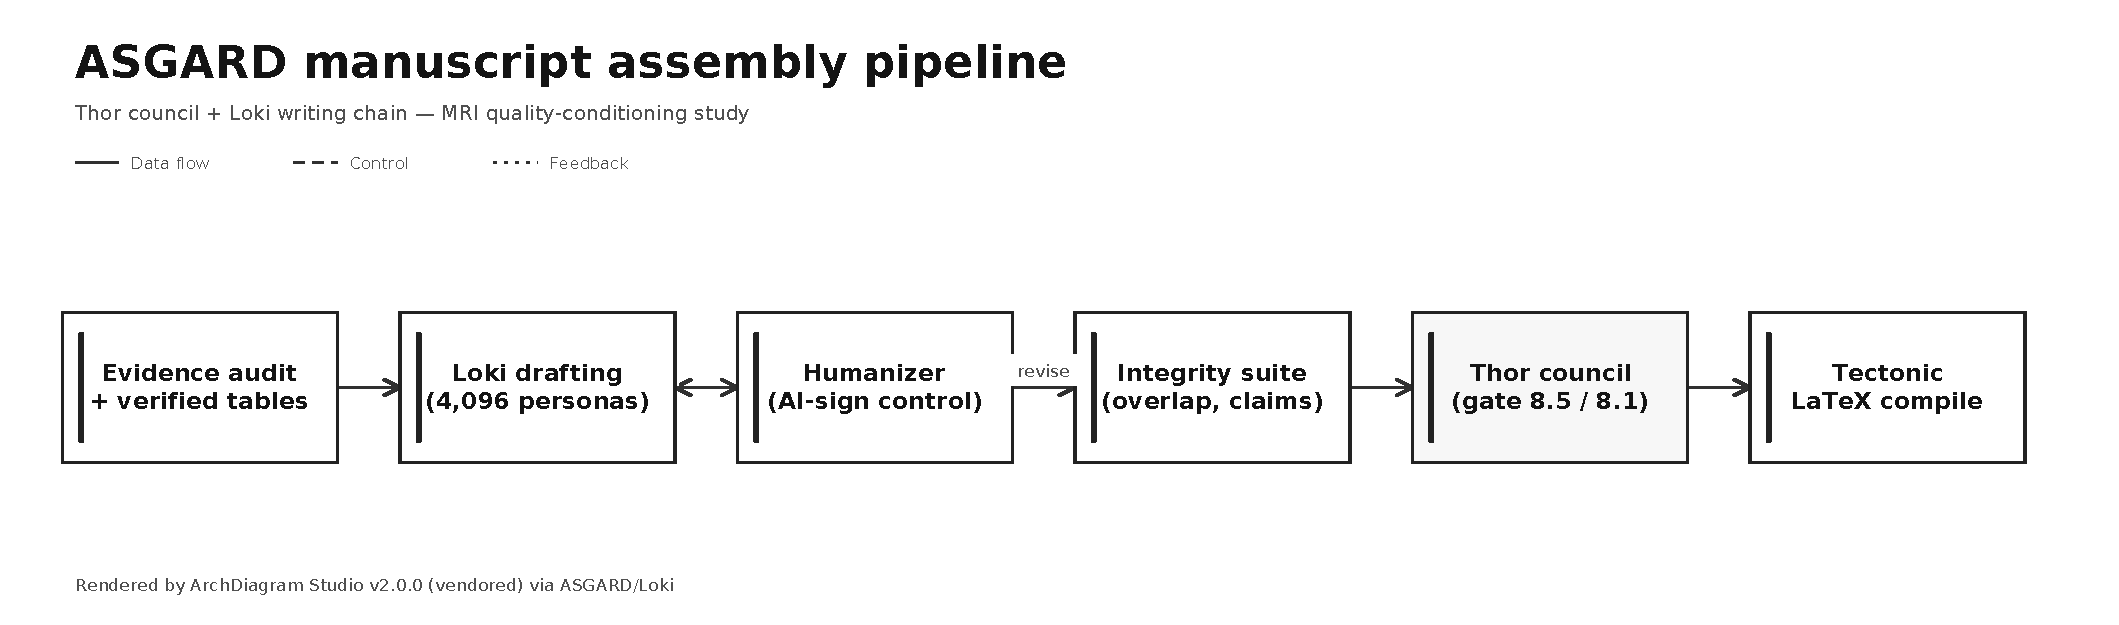
\includegraphics[width=\columnwidth]{figures/asgard_assembly.pdf}
\caption{Manuscript assembly pipeline rendered by the ASGARD diagram engine: audited evidence and verified tables feed section drafting under author personas; the humaniser and integrity suite gate the draft; the Thor council scores it against a fixed quality gate before compilation.}
\label{fig:assembly}
\end{figure}

